\documentclass[a4paper,12pt]{article}

%%% Работа с русским языком % для pdfLatex
\usepackage{cmap}					% поиск в~PDF
\usepackage{mathtext} 				% русские буквы в~фомулах
\usepackage[T2A]{fontenc}			% кодировка
\usepackage[utf8]{inputenc}			% кодировка исходного текста
\usepackage[english,russian]{babel}	% локализация и переносы
\usepackage{indentfirst} 			% отступ 1 абзаца

%%% Работа с русским языком % для XeLatex
%\usepackage[english,russian]{babel}   %% загружает пакет многоязыковой вёрстки
%\usepackage{fontspec}      %% подготавливает загрузку шрифтов Open Type, True Type и др.
%\defaultfontfeatures{Ligatures={TeX},Renderer=Basic}  %% свойства шрифтов по умолчанию
%\setmainfont[Ligatures={TeX,Historic}]{Times New Roman} %% задаёт основной шрифт документа
%\setsansfont{Comic Sans MS}                    %% задаёт шрифт без засечек
%\setmonofont{Courier New}
%\usepackage{indentfirst}
%\frenchspacing

%%% Дополнительная работа с математикой
\usepackage{amsfonts,amssymb,amsthm,mathtools}
\usepackage{amsmath}
\usepackage{icomma} % "Умная" запятая: $0,2$~--- число, $0, 2$~--- перечисление
\usepackage{upgreek}

%%% Страница
\usepackage{extsizes} % Возможность сделать 14-й шрифт

%% Шрифты
\usepackage{euscript}	 % Шрифт Евклид
\usepackage{mathrsfs} % Красивый матшрифт

%% Свои команды
\DeclareMathOperator{\sgn}{\mathop{sgn}} % создание новой конанды \sgn (типо как \sin)
\usepackage{csquotes} % ещё одна штука для цитат
\newcommand{\pd}[2]{\ensuremath{\cfrac{\partial #1}{\partial #2}}} % частная производная
\newcommand{\abs}[1]{\ensuremath{\left|#1\right|}} % модуль
\renewcommand{\phi}{\ensuremath{\varphi}} % греческая фи
\newcommand{\pogk}[1]{\!\left(\cfrac{\sigma_{#1}}{#1}\right)^{\!\!\!2}\!}

% Ссылки
\usepackage{color} % подключить пакет color
% выбрать цвета
\definecolor{BlueGreen}{RGB}{49,152,255}
\definecolor{Violet}{RGB}{120,80,120}
% назначить цвета при подключении hyperref
\usepackage[unicode, colorlinks, urlcolor=blue, linkcolor=blue, pagecolor=blue, citecolor=blue]{hyperref} %синие ссылки
%\usepackage[unicode, colorlinks, urlcolor=black, linkcolor=black, pagecolor=black, citecolor=black]{hyperref} % для печати (отключить верхний!)
\mathtoolsset{showonlyrefs=true} % Показывать номера только у тех формул, на которые есть \eqref{} в~тексте.


%% Перенос знаков в~формулах (по Львовскому)
\newcommand*{\hm}[1]{#1\nobreak\discretionary{}
	{\hbox{$\mathsurround=0pt #1$}}{}}

%%% Работа с картинками
\usepackage{graphicx}  % Для вставки рисунков
\graphicspath{{images/}{images2/}}  % папки с картинками
\setlength\fboxsep{3pt} % Отступ рамки \fbox{} от рисунка
\setlength\fboxrule{1pt} % Толщина линий рамки \fbox{}
\usepackage{wrapfig} % Обтекание рисунков и таблиц текстом
\usepackage{multicol}

%%% Работа с таблицами
\usepackage{array,tabularx,tabulary,booktabs} % Дополнительная работа с таблицами
\usepackage{longtable}  % Длинные таблицы
\usepackage{multirow} % Слияние строк в~таблице
\usepackage{caption}
\captionsetup{labelsep=period, labelfont=bf}

%%% Оформление
\usepackage{indentfirst} % Красная строка
%\setlength{\parskip}{0.3cm} % отступы между абзацами

%%% Теоремы
\theoremstyle{plain} % Это стиль по умолчанию, его можно не переопределять.
\newtheorem{theorem}{Теорема}[section]
\newtheorem{proposition}[theorem]{Утверждение}

\theoremstyle{definition} % "Определение"
\newtheorem{definition}{Определение}[section]
\newtheorem{corollary}{Следствие}[theorem]
\newtheorem{problem}{Задача}[section]

\theoremstyle{remark} % "Примечание"
\newtheorem*{nonum}{Решение}
\newtheorem{zamech}{Замечание}[theorem]

%%% Правильные мат. символы для русского языка
\renewcommand{\epsilon}{\ensuremath{\varepsilon}}
\renewcommand{\phi}{\ensuremath{\varphi}}
\renewcommand{\kappa}{\ensuremath{\varkappa}}
\renewcommand{\le}{\ensuremath{\leqslant}}
\renewcommand{\leq}{\ensuremath{\leqslant}}
\renewcommand{\ge}{\ensuremath{\geqslant}}
\renewcommand{\geq}{\ensuremath{\geqslant}}
\renewcommand{\emptyset}{\varnothing}


%%% Название разделов
\usepackage{titlesec}

\usepackage{graphicx}
\graphicspath{}
\DeclareGraphicsExtensions{.pdf,.png,.jpg}

\usepackage{titlesec}
\titleformat{\section}{\normalfont\Large\bfseries}{}{0pt}{}


\title{Отчет по лабораторной работе "Спектроскопия электронного парамагнитного резонанса."}
\author{Гадецкий Дмитрий}
\date{Март 2019}
\usepackage[left=1.35cm,right=1.35cm,top=1.4cm,bottom=2cm]{geometry}


\begin{document}
\maketitle
\thispagestyle{empty}
\newpage	 

\section{Ход работы и обработка данных}
\subsection{Влияние амплитуды высокочастотной модуляции на вид спектров ЭПР}

Были зарегистрированы спектры ЭПР ДФПГ при разных амплитудах
модуляции магнитного поля, изменялась величина тока в модуляционных
катушках.
Видно, что с увеличением амплитуды модуляции
амплитуда сигнала и расстояние между экстремумами увеличивается.

\begin{figure}[h!]
	\centering{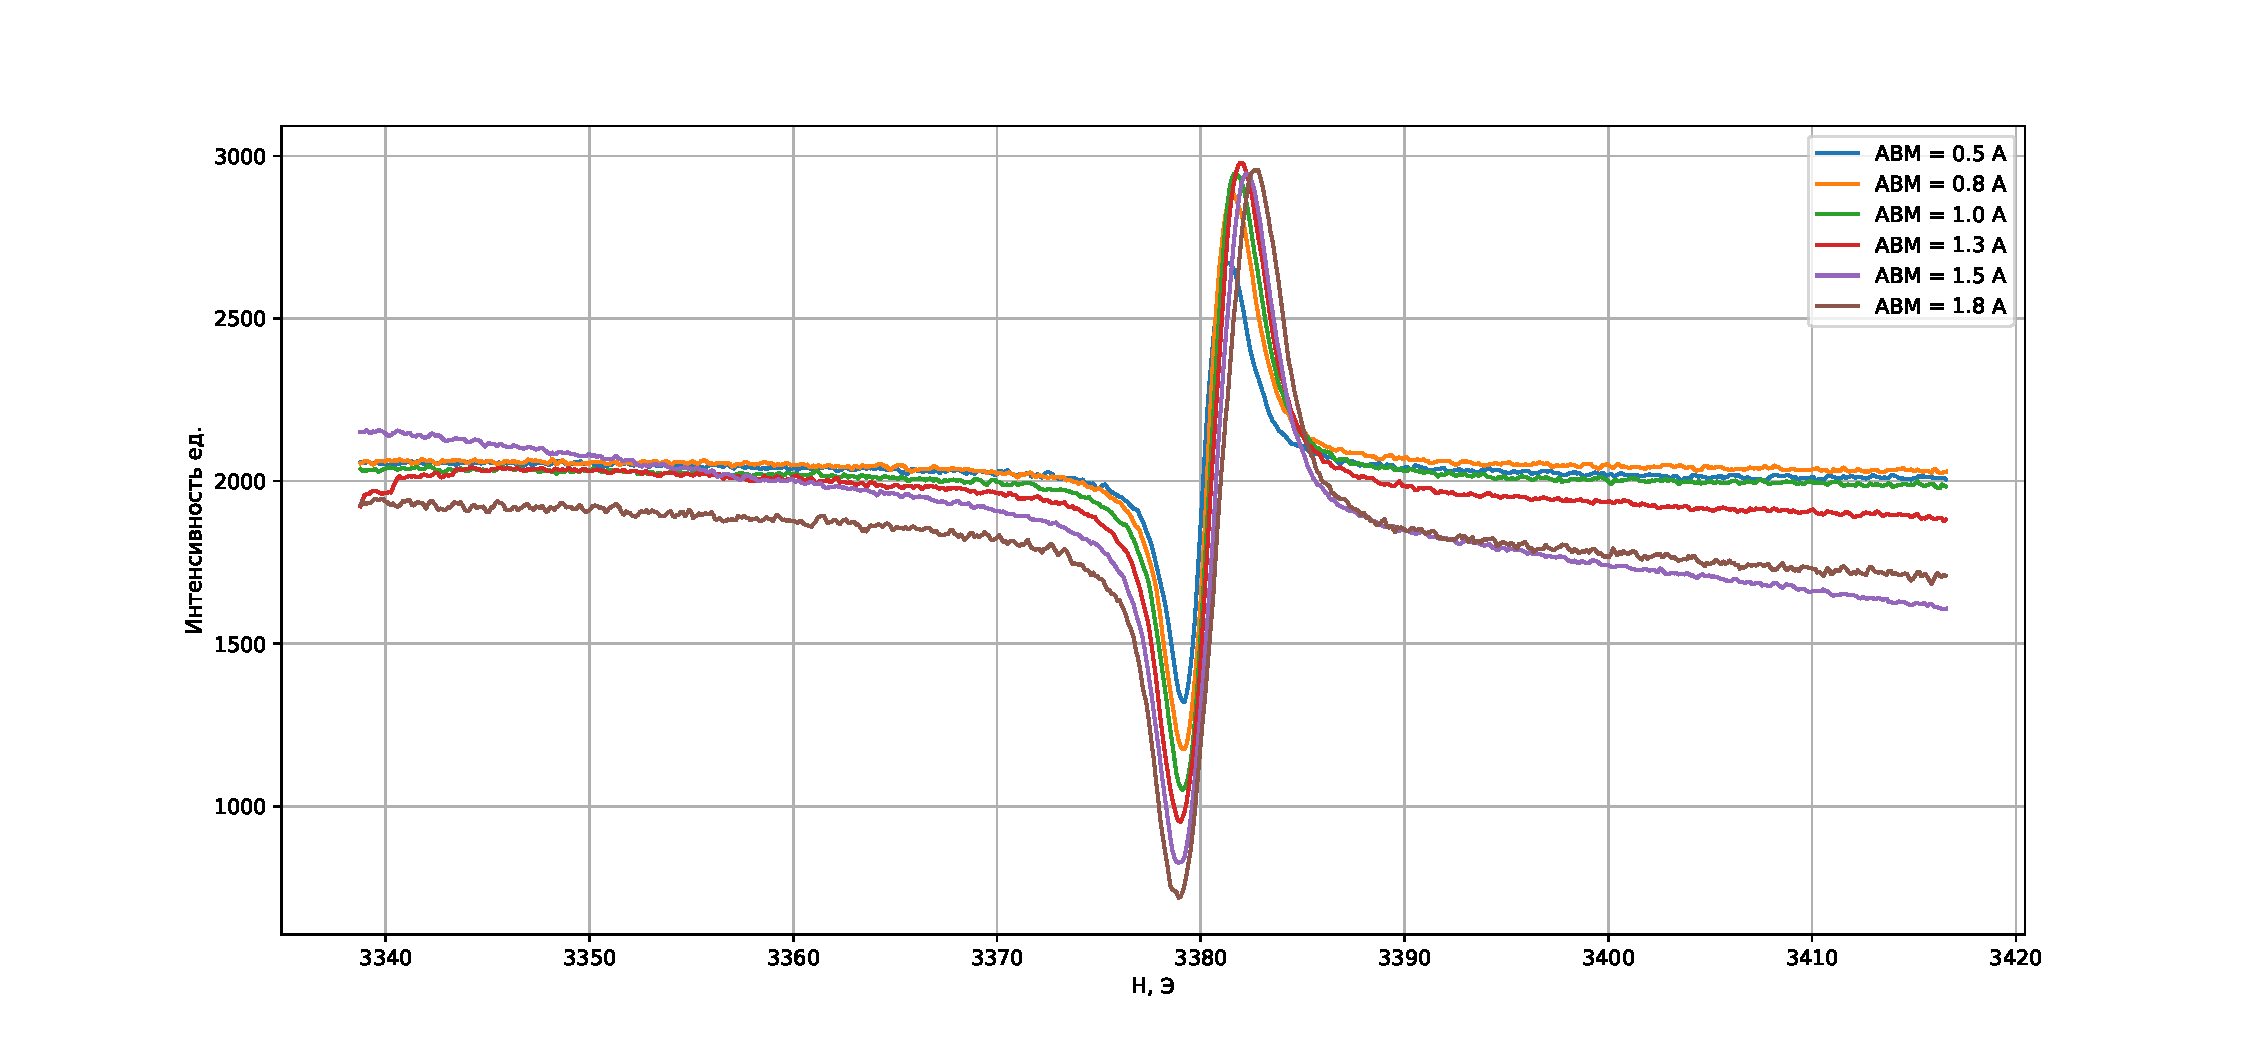
\includegraphics[scale=0.5]{fig1.pdf}}
	\caption{спектры ЭПР ДФПГ (Зависимость от АВМ)}
	\label{fig:image}
\end{figure}

Были рассчитаны полуширины линий поглощения $\delta H$ для каждой величины
тока модуляции и далее приводится их зависмость от величины тока модуляции.

\begin{figure}[h!]
	\centering{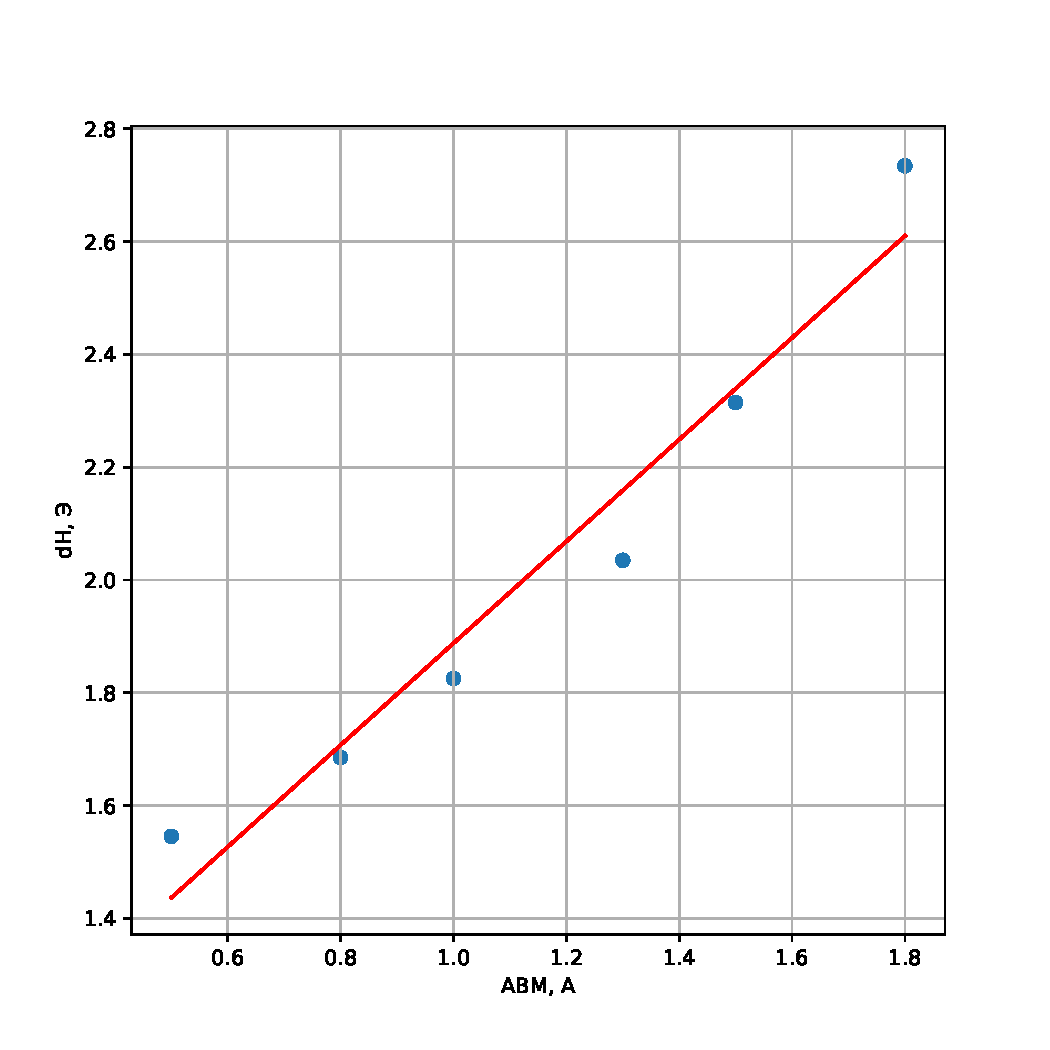
\includegraphics[scale=0.5]{fig2.pdf}}
	\caption{Зависимость $\delta H$ линий поглощения от величины тока модуляции}
	\label{fig:image}
\end{figure}

\newpage

Максимальная амплитуда модуляции, для рассчета которой использовался коэффициент наклона прямой (Рис. 2.) ,
оказалась равной $(0.99 \pm 0.07)$ Э.

\subsection{Исследование скорости спинового обмена в растворах и кристаллах}
Были зарегистрированы спектры ЭПР при разных концентрациях соли $Mn^{2+}$. 


\begin{figure}[h!]
	\centering{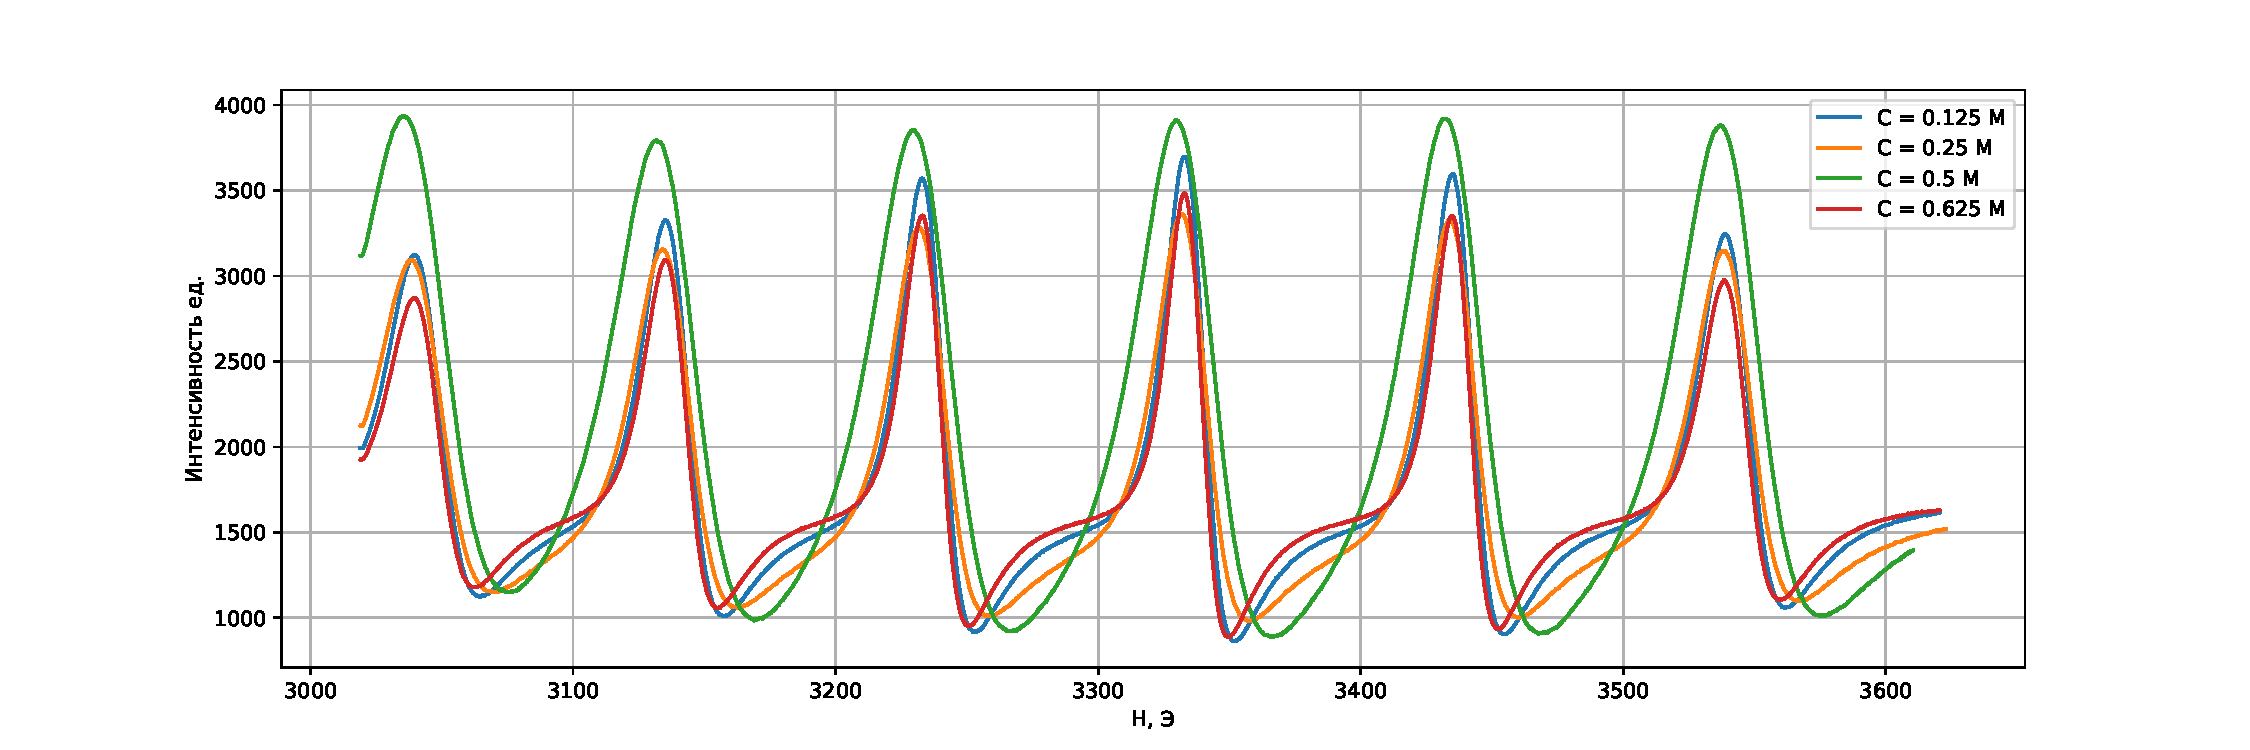
\includegraphics[scale=0.5]{fig3.pdf}}
	\caption{Спектры ЭПР раствора $Mn^{2+}$ при разной концентрации}
	\label{fig:image}
\end{figure}

C увеличением концентрации уменьшается амплитуда сигнала, но положения экстремумов остаётся практически теми же.
Что касается концентрации в $0.5$ M -- просто использовался другой коэффициент усиления.
Далее привожу график зависимости полуширины линии поглощения $\delta $ от концентрации раствора. Измерения провожу по 
крайнему правому пику.

\begin{figure}[h!]
	\centering{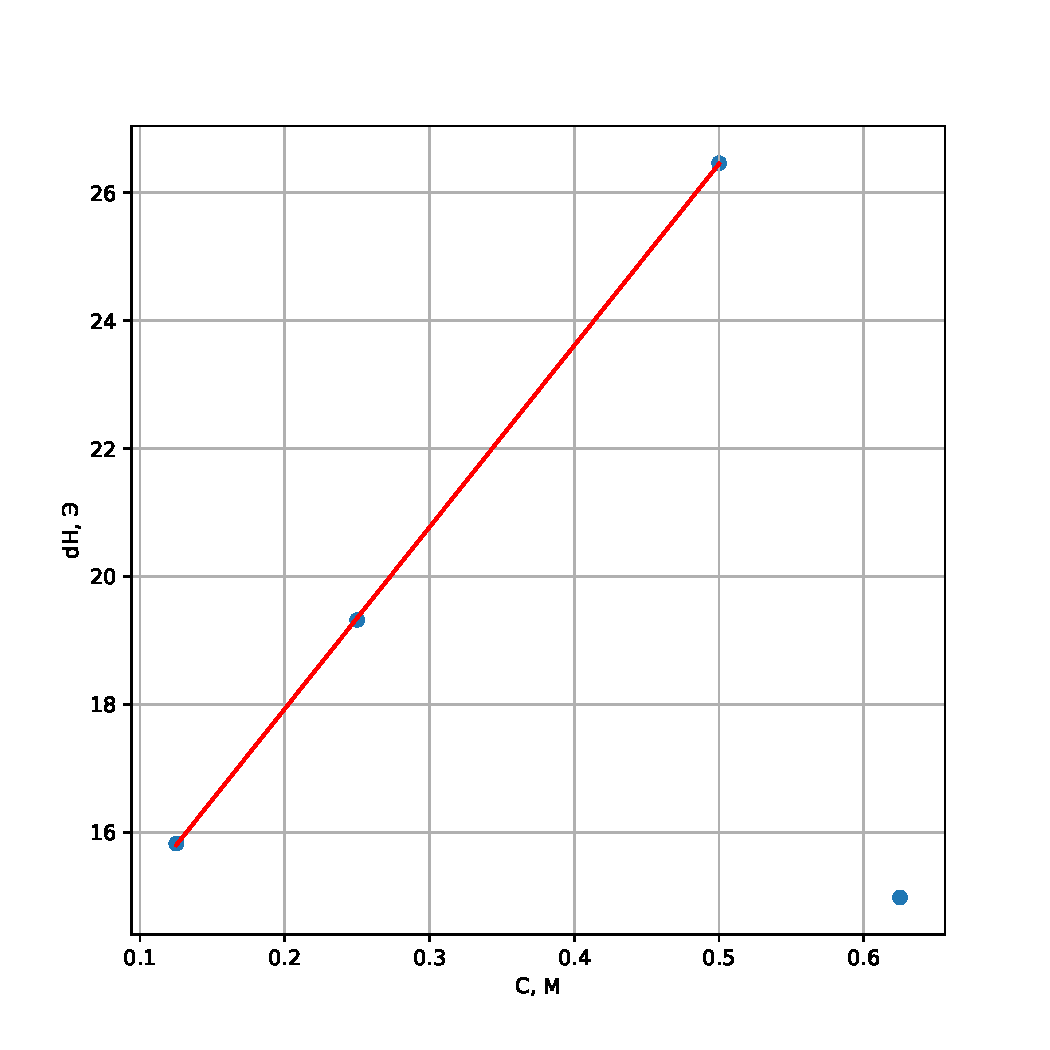
\includegraphics[scale=0.5]{fig4.pdf}}
	\caption{Зависимость полуширины линии
		поглощения от концентрации
		раствора}
	\label{fig:image}
\end{figure}

Одну точку после неоднократной перепроверки вычислений пришлось убрать из дальнейшего рассмотрения.
По наклону полученной прямой (Рис. 4.) определяем константу спинового обмена $K_e $ :

\begin{equation}
	K_e = 4.9 \cdot 10^8 \pm 10^{7} M^{-1}c^{-1}
\end{equation}

\newpage

Далее просто привожу характерный порядок частоты столкновений парамагнитных частиц в растворе:

\begin{equation}
\frac{1}{\tau} = K_e \cdot C \approx 2.5 \cdot 10^8 Hz
\end{equation}

На (Рис. 5.) представлен спектр ЭПР сухого порошка $Mn^{2+}$.

\begin{figure}[h!]
	\centering{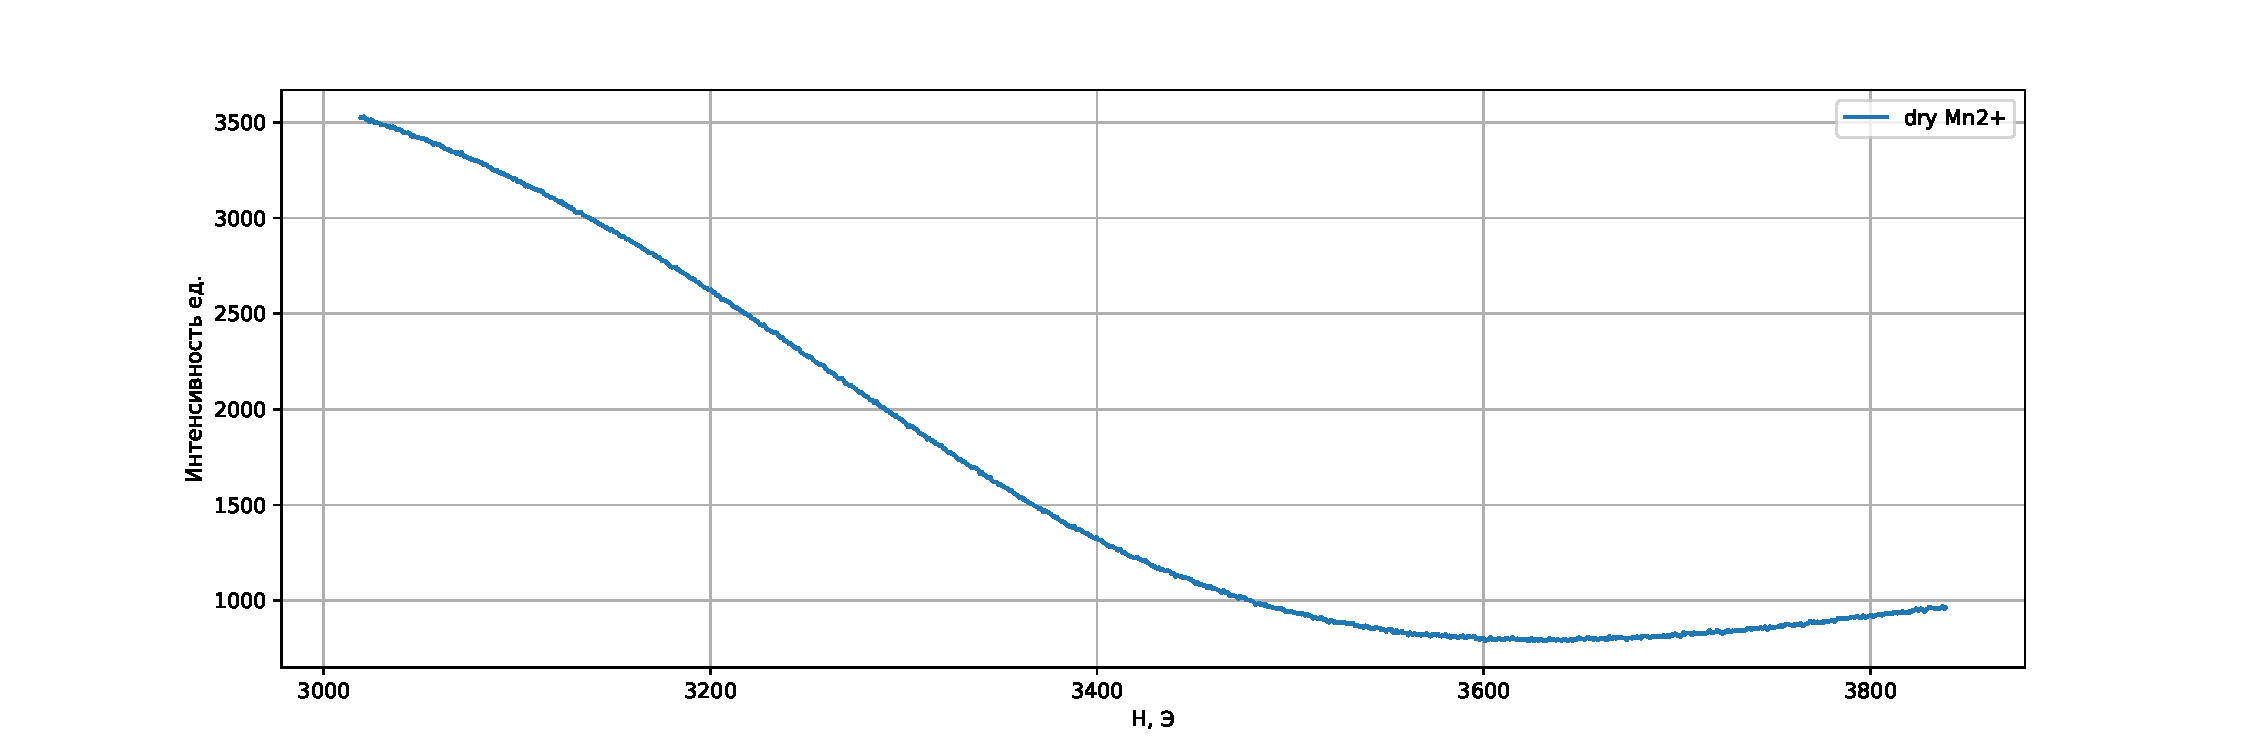
\includegraphics[scale=0.5]{fig5.pdf}}
	\caption{Спектр ЭПР для сухого порошка MnCl2}
	\label{fig:image}
\end{figure}

Можно сделать следующие качественные выводы:
\\
1) В растворе наблюдаем случай медленного спинового обмена. Скорость
обмена увеличивается с увеличением концентрации
\\
2)  Для кристаллического марганца
имеем случай быстрого спинового обмена, наблюдаем что пики усредняются
и сливаются в один.

\subsection{Исследование сверхтонкой структуры спектров  ЭПР.}

Сначала определим константу сверхтонкого взаимодействия как расстояние между 
эквидистантными пиками для ионов $Mn^{2+}$. 

\begin{equation}
	a = 100.4 \pm 0.1 \hspace{1 mm} \text{Э}
\end{equation}

Далее будем наблюдать ЭПР спектр порошка мела:

\begin{figure}[h!]
	\centering{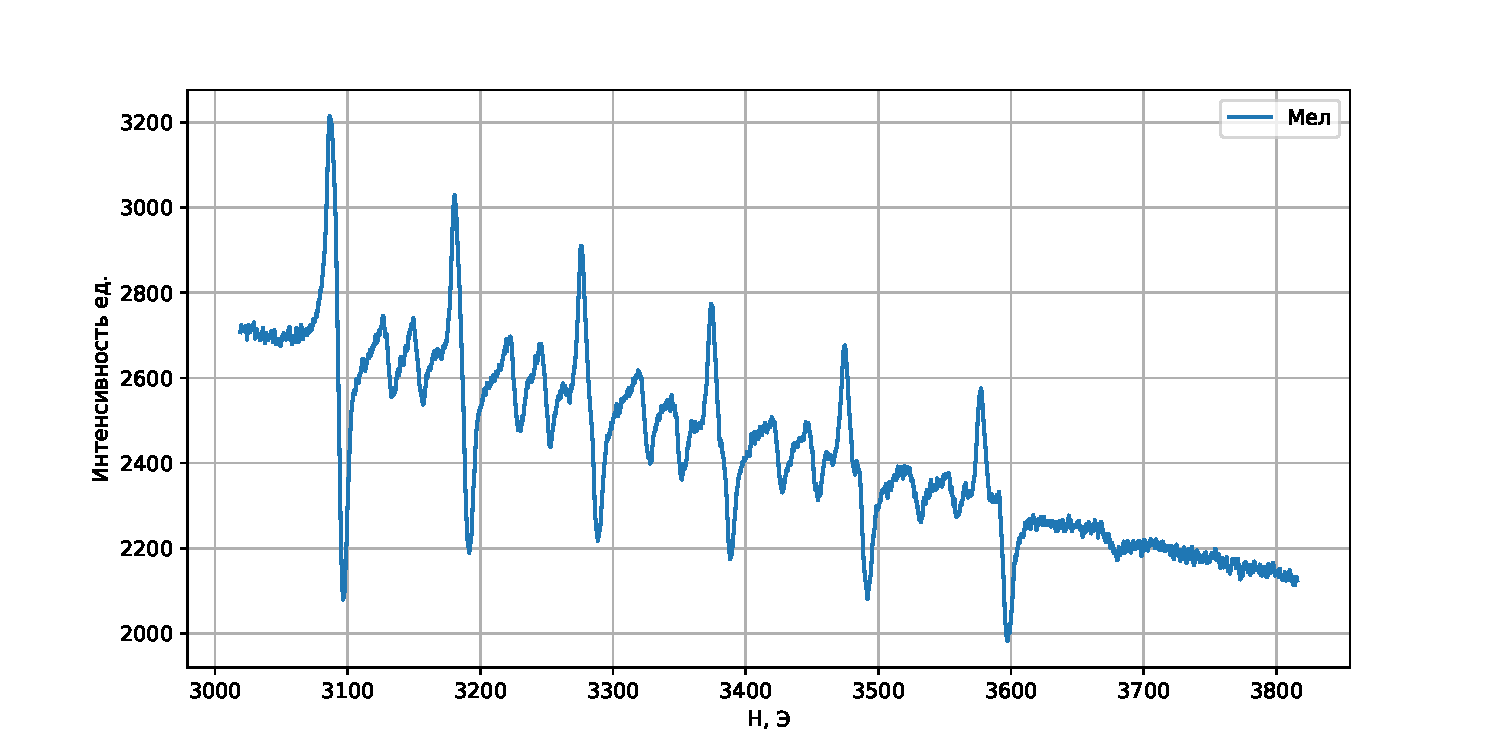
\includegraphics[scale=0.5]{fig6.pdf}}
	\caption{Спектр ЭПР порошка мела}
	\label{fig:image}
\end{figure}

\newpage

В ЭПР спектре мела можно увидеть 6 линий поглощения. Причиной такого количества линий 
может являться ядро со спином $5/2$, это может быть изотоп кислорода $^{17}O$ входящий в карбонат 
кальция. Доля $^{17}O$ в природе -- $0.038 \hspace{1 mm}\%$.

\begin{figure}[h!]
	\centering{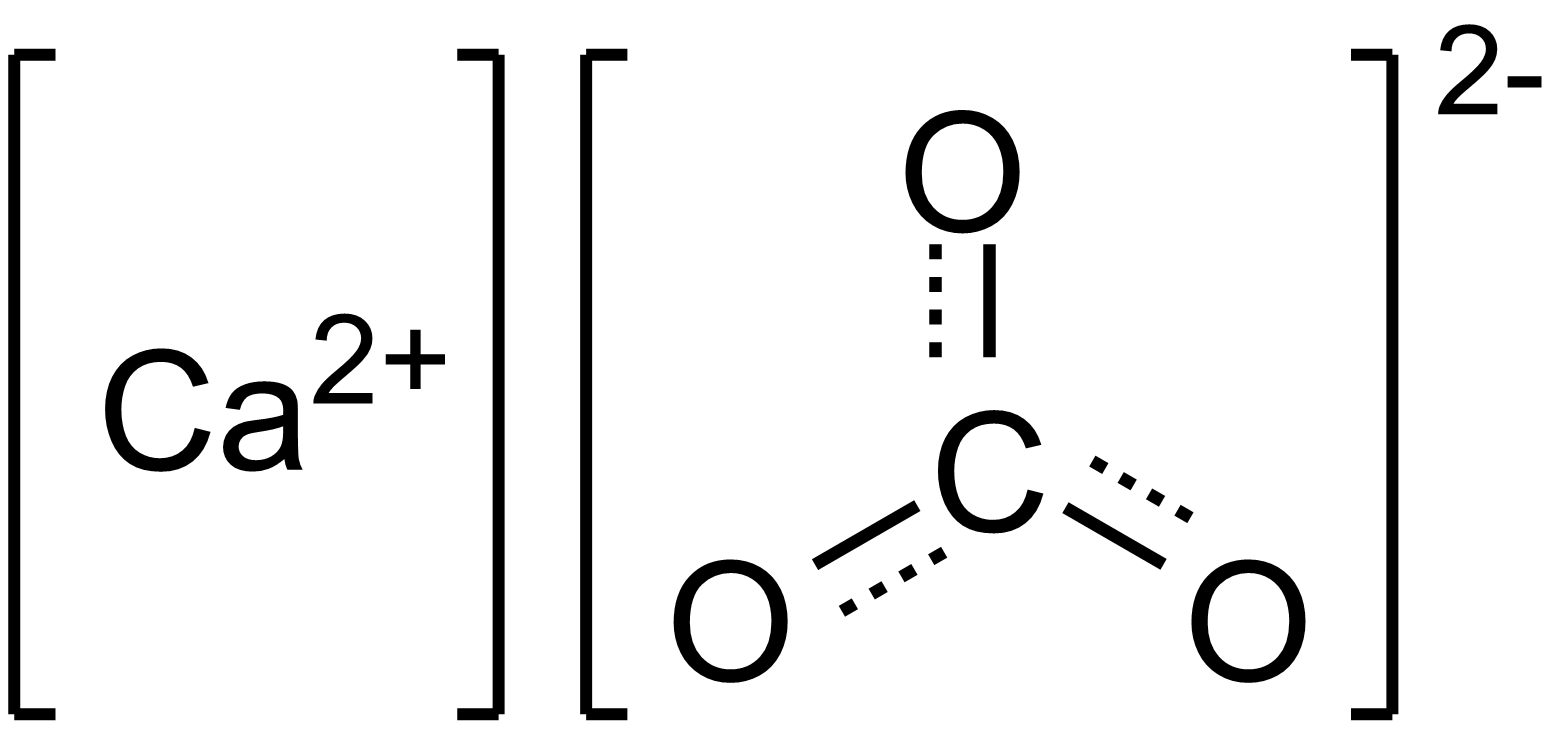
\includegraphics[scale=0.2]{cc.png}}
	\caption{Карбонат кальция}
	\label{fig:image}
\end{figure}

\subsection{Исследование влияния диэлектрических потерь на вид спектров ЭПР}

Были измерены спектры ЭПР для растворов $Mn^{2+}$ низкой концентрации:
\\
a) в капилляре
\\б) в пробирке, сохраняя ту же высоту столба жидкости, что и в пункте а.
\\в) в пробирке, сохраняя то же количество парамагнитных центров,что и в пункте а и при таком же объёме, как в пункте б.

\begin{figure}[h!]
	\centering{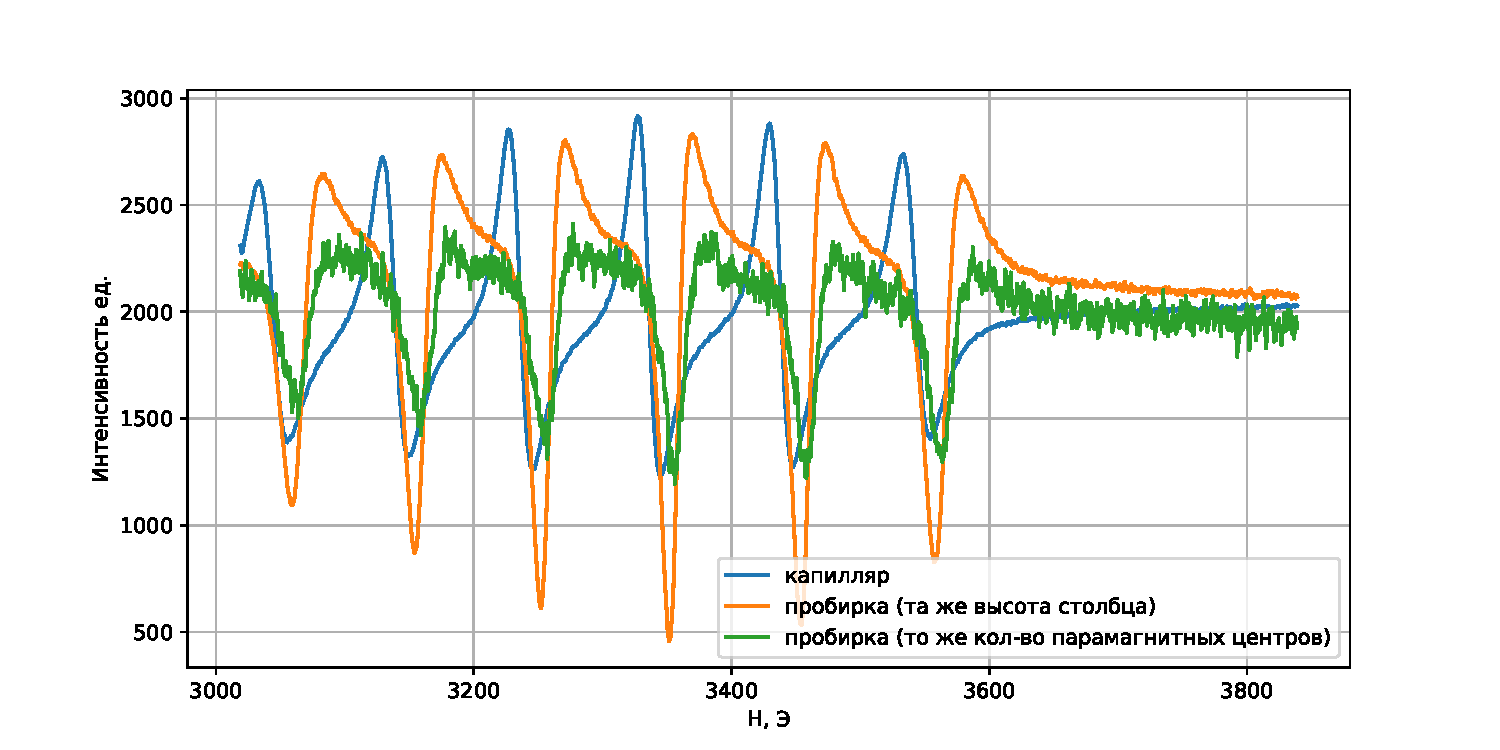
\includegraphics[scale=0.7]{fig7.pdf}}
	\caption{Спектр ЭПР $Mn^{2+}$}
	\label{fig:image}
\end{figure}

Анализ:
\\
В случае a:\\
Уровень диамагнитных потерь наименьший.
\\В случае б:
\\ В пробирке должно быть больше парамагнитных центров, уровень диамагнитных 
потерь наибольший.
\\В случае в:
\\Число парамагнитных центров осталось тем
же, но амплитуда сигнала уменьшилась из-за увеличения диаметра
сосуда с образцом.

\newpage

\subsection{Выводы}
$\text{}$
\\1)Было установлено, что увеличение амплитуды модуляции помимо уменьшения
шумов на спектре, приводит к уширению пиков. Оптимальная
величина тока модуляции оказалась равной 1 А.
\\ \\
2)Было установлено, что увеличение концентрации раствора $Mn^{2+}$
увеличивает скорость спинового обмена, уширяя пики.\\\\
3) Для катионов $Mn^{2+}$ было измерено значение константы спинового обмена. $K_e = 4.9\cdot 10^8 \pm 10^7 M^{-1}c^{-1} $ 
\\\\4)
Была определена константа сверхтонкого взаимодействия для раствора $Mn^{2+}$ ($a = 100.4 \pm 0.1$) Э.
\\\\5)Было продемонстрировано ухудшение сигнала при сильном разбавлении
и увеличении объёма образца.
\end{document}

Далее 